\clearpage



\begin{appendix}
\clearpage
\appendix

\hypertarget{data-generation-procedure}{%
\section{\texorpdfstring{Data Generation Procedure
\label{app:data-generation}}{Data Generation Procedure }}\label{data-generation-procedure}}

All data processing was conducted in R statistical software. A total of
\(N = 30\) points \((x_i, y_i), i = 1,...N\) were generated for
\(x_i \in [x_{min}, x_{max}]\) where \(x\) and \(y\) have a linear
relationship. Data were simulated based on a linear model with additive
errors: \begin{align}
y_i & = \beta_0 + \beta_1 x_i + e_i \\
\text{with } e_i & \sim N(0, \sigma^2). \nonumber
\end{align}

Model equation parameters, \(\beta_0\) and \(\beta_1\), were selected to
reflect the four data sets (F, N, S, and V) used in Mosteller, Siegel,
Trapido, \& Youtz (1981) \pcref{tab:eyefitting-parameters}. Parameter
choices F, N, and S simulated data across a domain of 0 to 20. Parameter
choice F produces a trend with a positive slope and a large variance
while N has a negative slope and a large variance. In comparison, S
shows a trend with a positive slope with a small variance and V yields a
steep positive slope with a small variance over the domain of 4 to 16.
\cref{fig:eyefitting-simplot} illustrates an example of simulated data
for all four parameter choices intended to reflect the trends in
Mosteller, Siegel, Trapido, \& Youtz (1981). Aesthetic design choices
were made consistent across each of the interactive `You Draw It' task
plots. The y-axis range extended 10\% beyond (above and below) the range
of the simulated data points to allow for users to draw outside the
simulated data set range.

\begin{table}

\caption{\label{tab:eyefitting-parameters}Designated model equation parameters for simulated data.}
\centering
\begin{tabular}[t]{cccc}
\toprule
Parameter Choice & $y_{\bar{x}}$ & $\beta_1$ & $\sigma$\\
\midrule
S & 3.88 & 0.66 & 1.30\\
F & 3.90 & 0.66 & 1.98\\
V & 3.89 & 1.98 & 1.50\\
N & 4.11 & -0.70 & 2.50\\
\bottomrule
\end{tabular}
\end{table}

\begin{figure}

{\centering 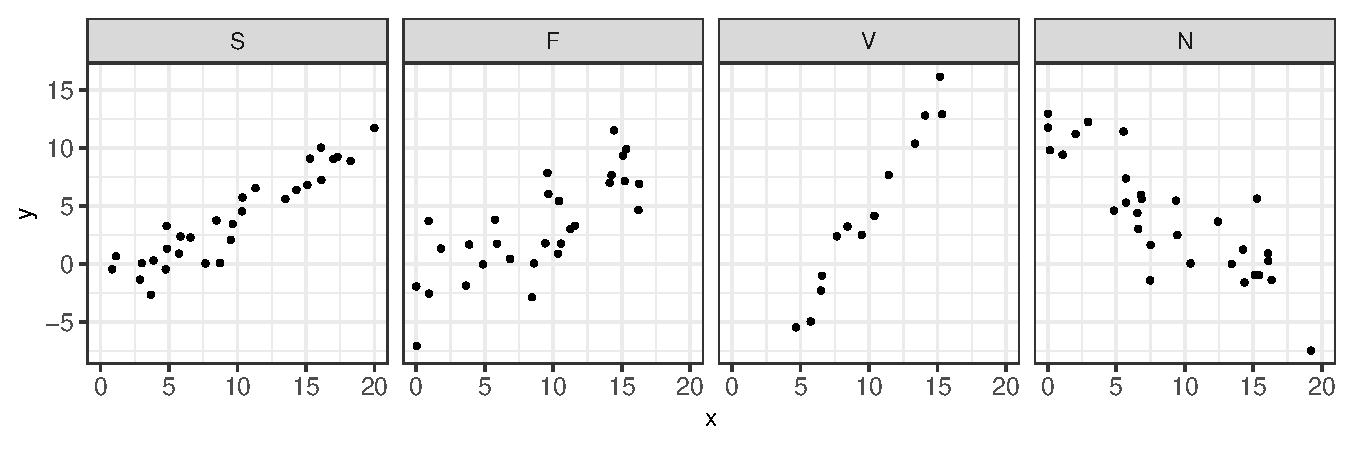
\includegraphics[width=1\linewidth]{./images/eyefitting-simplot-1} 

}

\caption{Example of simulated data points displayed in a scatter-plot illustrating the trends associated with the four selected parameter choices.}\label{fig:eyefitting-simplot}
\end{figure}

\hypertarget{fitted-regression-lines}{%
\section{\texorpdfstring{Fitted Regression Lines
\label{app:fitted-regression}}{Fitted Regression Lines }}\label{fitted-regression-lines}}

We compare the participant drawn line to two regression lines determined
by ordinary least squares regression and regression based on the
principal axis (i.e.~Deming Regression). \cref{fig:ols-vs-pca-example}
illustrates the difference between an OLS regression line which
minimizes the vertical distance of points from the line and a regression
line based on the principal axis which minimizes the Euclidean distance
of points (orthogonal) from the line.

Due to the randomness in the data generation process, the actual slope
of the linear regression line fit through the simulated points could
differ from the predetermined slope. Therefore, we fit an ordinary least
squares (OLS) regression to each scatter-plot to obtain estimated
parameters \(\hat\beta_{0,OLS}\) and \(\hat\beta_{1,OLS}\). Fitted
values, \(\hat y_{k,OLS}\), are then obtained every 0.25 increments
across the domain from the OLS regression equation,
\(\hat y_{k,OLS} = \hat\beta_{0,OLS} + \hat\beta_{1,OLS} x_k\)., for
\(k = 1, ..., 4 x_{max} +1\). The regression equation based on the
principal axis was determined by using the \texttt{princomp} function in
the stats package in base R to obtain the rotation of the coordinate
axes from the first principal component (direction which captures the
most variance). The estimated slope, \(\hat\beta_{1,PCA}\), is
determined by the ratio of the axis rotation in y and axis rotation in x
of the first principal component with the y-intercept,
\(\hat\beta_{0,PCA}\) calculated by the point-slope equation of a line
using the mean of of the simulated points, \((\bar x_i, \bar y_i)\).
Fitted values, \(\hat y_{k,PCA}\), are then obtained every 0.25
increment across the domain from the PCA regression equation,
\(\hat y_{k,PCA} = \hat\beta_{0,PCA} + \hat\beta_{1,PCA} x_k\).

\begin{figure}

{\centering 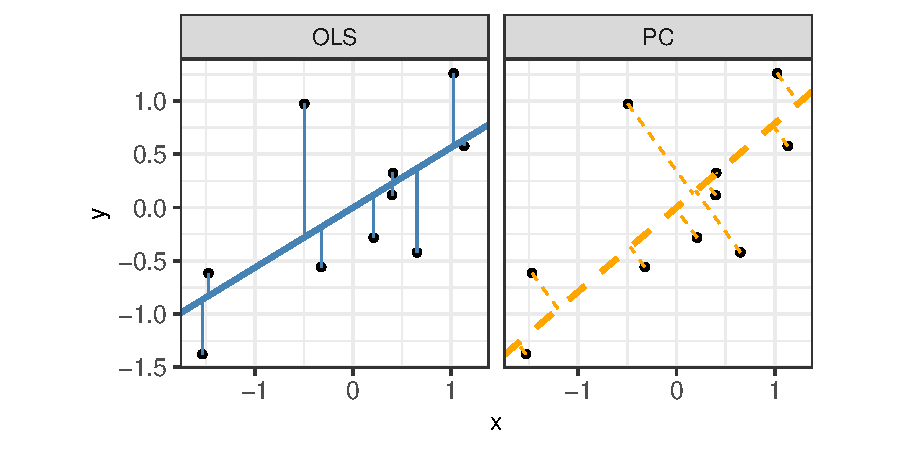
\includegraphics[width=0.9\linewidth]{./images/ols-vs-pca-example-1} 

}

\caption{ Comparison between an OLS regression line which minimizes the vertical distance of points from the line and a regression line based on the principal axis which minimizes the Euclidean distance of points (orthogonal) from the line.}\label{fig:ols-vs-pca-example}
\end{figure}

\hypertarget{residual-trends}{%
\section{\texorpdfstring{Residual Trends
\label{app:residual-trends}}{Residual Trends }}\label{residual-trends}}

For each participant, the final data set used for analysis contains
\(x_{ijk}, y_{ijk,drawn}, \hat y_{ijk,OLS}\), and \(\hat y_{ijk,PCA}\)
for parameter choice \(i = 1,2,3,4\), j = \(1,...N_{participant}\), and
\(x_{ijk}\) value \(k = 1, ...,4 x_{max} + 1\). Using both a linear
mixed model and a generalized additive mixed model, comparisons of
vertical residuals in relation to the OLS fitted values
(\(e_{ijk,OLS} = y_{ijk,drawn} - \hat y_{ijk,OLS}\)) and PCA fitted
values (\(e_{ijk,PCA} = y_{ijk,drawn} - \hat y_{ijk,PCA}\)) were made
across the domain. \cref{fig:eyefitting-example-plot} displays an
example of all three fitted trend lines for parameter choice F. Data
used in the analyses are available to be downloaded from GitHub
\href{https://github.com/earobinson95/Eye-Fitting-Straight-Lines-in-the-Modern-Era/raw/main/data/youdrawit-eyefitting-model-data.csv}{here}.

\begin{figure}

{\centering 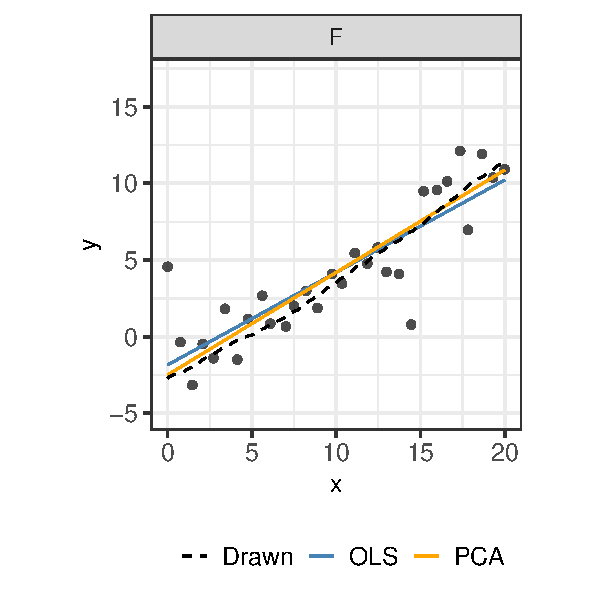
\includegraphics[width=0.75\linewidth]{./images/eyefitting-example-plot-1} 

}

\caption{Illustrates the data associated with and collected for one 'You Draw It' task plot. Trend-lines include the participant drawn line (dashed black), the OLS regression line (solid steelblue) and the PCA regression line based on the principal axis (solid orange).}\label{fig:eyefitting-example-plot}
\end{figure}

\hypertarget{linear-mixed-model}{%
\subsection{\texorpdfstring{Linear Mixed Model
\label{app:lmm-equation}}{Linear Mixed Model }}\label{linear-mixed-model}}

Using the \texttt{lmer} function in the lme4 package (Bates, Mächler,
Bolker, \& Walker, 2015), a linear mixed model (LMM) is fit separately
to the OLS residuals and PCA residuals, constraining the fit to a linear
trend. Parameter choice, \(x\), and the interaction between \(x\) and
parameter choice were treated as fixed effects with a random participant
effect accounting for variation due to participant. The LMM equation for
each fit (OLS and PCA) is given by: \begin{equation}
e_{ijk,fit} = \left[\gamma_0 + \alpha_i\right] + \left[\gamma_{1} x_{ijk} + \gamma_{2i} x_{ijk}\right] + p_{j} + \epsilon_{ijk}
\end{equation} \noindent where

\begin{itemize}
\tightlist
\item
  \(y_{ijk,drawn}\) is the drawn y-value for the \(i^{th}\) parameter
  choice, \(j^{th}\) participant, and \(k^{th}\) increment of x-value
\item
  \(\hat y_{ijk,fit}\) is the fitted y-value for the \(i^{th}\)
  parameter choice, \(j^{th}\) participant, and \(k^{th}\) increment of
  x-value corresponding to either the OLS or PCA fit
\item
  \(e_{ijk,fit}\) is the residual between the drawn and fitted y-values
  for the \(i^{th}\) parameter choice, \(j^{th}\) participant, and
  \(k^{th}\) increment of x-value corresponding to either the OLS or PCA
  fit
\item
  \(\gamma_0\) is the overall intercept
\item
  \(\alpha_i\) is the effect of the \(i^{th}\) parameter choice (F, S,
  V, N) on the intercept
\item
  \(\gamma_1\) is the overall slope for \(x\)
\item
  \(\gamma_{2i}\) is the effect of the parameter choice on the slope
\item
  \(x_{ijk}\) is the x-value for the \(i^{th}\) parameter choice,
  \(j^{th}\) participant, and \(k^{th}\) increment
\item
  \(p_{j} \sim N(0, \sigma^2_{participant})\) is the random error due to
  the \(j^{th}\) participant's characteristics
\item
  \(\epsilon_{ijk} \sim N(0, \sigma^2)\) is the residual error.
\end{itemize}

\hypertarget{generalized-additive-mixed-model}{%
\subsection{\texorpdfstring{Generalized Additive Mixed Model
\label{app:gamm-equation}}{Generalized Additive Mixed Model }}\label{generalized-additive-mixed-model}}

Eliminating the linear trend constraint, the \texttt{bam} function in
the mgcv package (Wood, 2011) is used to fit a generalized additive
mixed model (GAMM) separately to the OLS residuals and PCA residuals to
allow for estimation of smoothing splines. Parameter choice was treated
as a fixed effect with no estimated intercept and a separate smoothing
spline for \(x\) was estimated for each parameter choice. A random
participant effect accounting for variation due to participant and a
random spline for each participant accounted for variation in spline for
each participant. The GAMM equation for each fit (OLS and PCA) residuals
is given by: \begin{equation}
e_{ijk,fit} = \alpha_i + s_{i}(x_{ijk}) + p_{j} + s_{j}(x_{ijk})
\end{equation} \noindent where

\begin{itemize}
\tightlist
\item
  \(y_{ijk,drawn}\) is the drawn y-value for the \(i^{th}\) parameter
  choice, \(j^{th}\) participant, and \(k^{th}\) increment of x-value
\item
  \(\hat y_{ijk,fit}\) is the fitted y-value for the \(i^{th}\)
  parameter choice, \(j^{th}\) participant, and \(k^{th}\) increment of
  x-value corresponding to either the OLS or PCA fit
\item
  \(e_{ijk,fit}\) is the residual between the drawn and fitted y-values
  for the \(i^{th}\) parameter choice, \(j^{th}\) participant, and
  \(k^{th}\) increment of x-value corresponding to either the OLS or PCA
  fit
\item
  \(\alpha_i\) is the intercept for the parameter choice \(i\)
\item
  \(s_{i}\) is the smoothing spline for the \(i^{th}\) parameter choice
\item
  \(x_{ijk}\) is the x-value for the \(i^{th}\) parameter choice,
  \(j^{th}\) participant, and \(k^{th}\) increment
\item
  \(p_{j} \sim N(0, \sigma^2_{participant})\) is the error due to
  participant variation
\item
  \(s_{j}\) is the random smoothing spline for each participant.
\end{itemize}
\end{appendix}
